\documentclass[14pt]{extbook}
\usepackage{multicol, enumerate, enumitem, hyperref, color, soul, setspace, parskip, fancyhdr} %General Packages
\usepackage{amssymb, amsthm, amsmath, latexsym, units, mathtools} %Math Packages
\everymath{\displaystyle} %All math in Display Style
% Packages with additional options
\usepackage[headsep=0.5cm,headheight=12pt, left=1 in,right= 1 in,top= 1 in,bottom= 1 in]{geometry}
\usepackage[usenames,dvipsnames]{xcolor}
\usepackage{dashrule}  % Package to use the command below to create lines between items
\newcommand{\litem}[1]{\item#1\hspace*{-1cm}\rule{\textwidth}{0.4pt}}
\pagestyle{fancy}
\lhead{Module4}
\chead{}
\rhead{Version A}
\lfoot{4485-7686}
\cfoot{}
\rfoot{test}
\begin{document}

\begin{enumerate}
\item{
Write the equation of the graph presented below in the form $f(x)=ax^2+bx+c$, assuming  $a=1$ or $a=-1$.
\begin{center}
    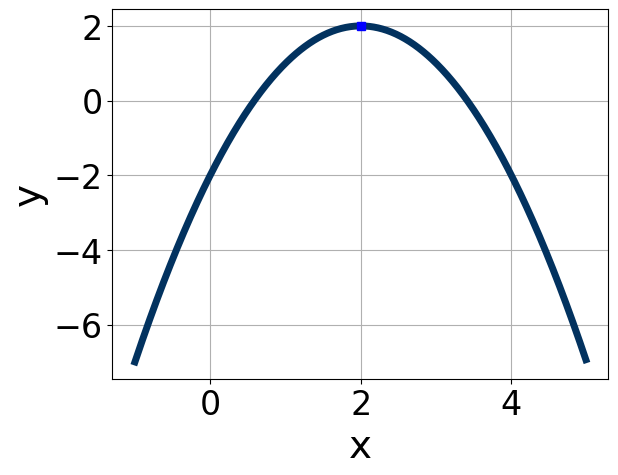
\includegraphics[width=0.5\textwidth]{../Figures/quadraticGraphToEquationCopyA.png}
\end{center}
} \newpage
\item{
Write the equation of the graph presented below in the form $f(x)=ax^2+bx+c$, assuming  $a=1$ or $a=-1$.
\begin{center}
    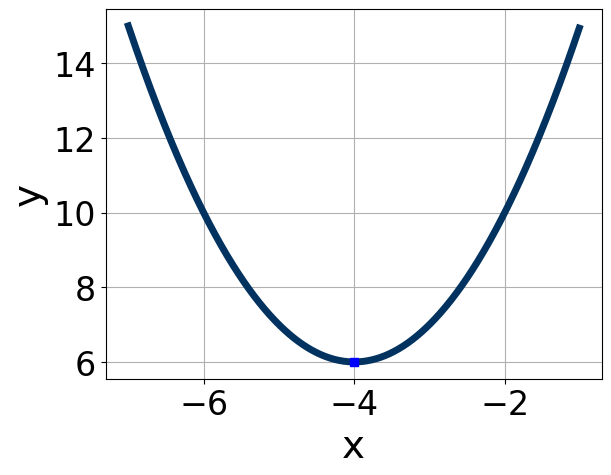
\includegraphics[width=0.5\textwidth]{../Figures/quadraticGraphToEquationA.png}
\end{center}
} \newpage
\item{
Solve the quadratic equation below.\[ 17x^{2} -13 x -5 = 0 \]} \newpage
\item{
Solve the quadratic equation below.\[ 25x^{2} +60 x + 36 = 0 \]} \newpage
\item{
Factor the quadratic below into the form $(ax+b)(cx+d)$.\[ 81x^{2} -18 x -8 \]} \newpage
\item{
Graph the equation below.\[ f(x) = -(x+4)^2 + 14 \]} \newpage
\item{
Graph the equation below.\[ f(x) = -(x+2)^2 - 10 \]} \newpage
\item{
Solve the quadratic equation below.\[ -17x^{2} +15 x + 4 = 0 \]} \newpage
\item{
Factor the quadratic below into the form $(ax+b)(cx+d)$.\[ 24x^{2} +38 x + 15 \]} \newpage
\item{
Solve the quadratic equation below.\[ 10x^{2} -57 x + 54 = 0 \]} \newpage
\end{enumerate}

\end{document}